\documentclass{article}

\usepackage[top=2cm, bottom=2cm, left=2cm, right=2cm]{geometry}
\usepackage{longtable}
\usepackage{graphicx}
\usepackage{hyperref}
\hypersetup{
	colorlinks=true,
	linkcolor=blue,
	filecolor=magenta,      
	urlcolor=cyan,
}

 \usepackage{booktabs}

\providecommand{\tightlist}{%
	\setlength{\itemsep}{0pt}\setlength{\parskip}{0pt}}

\title{Irritating Crusader}
\author{Pipat Saengow (id: 6232024821) \and Siri Thammarerkrit (id: 6232029021) }

\begin{document}

\vfill

\begin{LARGE}
\maketitle	
\end{LARGE}
	

	
\begin{center}

\large

\textbf{Team}: ProgMethMyFirstGame

\vspace{3cm}
	
\textbf{Submitted for}

Programming Methodology I (id: 2110215)

Semester II of 2019.

Final project presentation

\end{center}

\vfill

\pagebreak

\vfill
\tableofcontents
\vfill
\pagebreak

\hypertarget{overview}{%
\section{Overview}\label{overview}}

\begin{figure}
	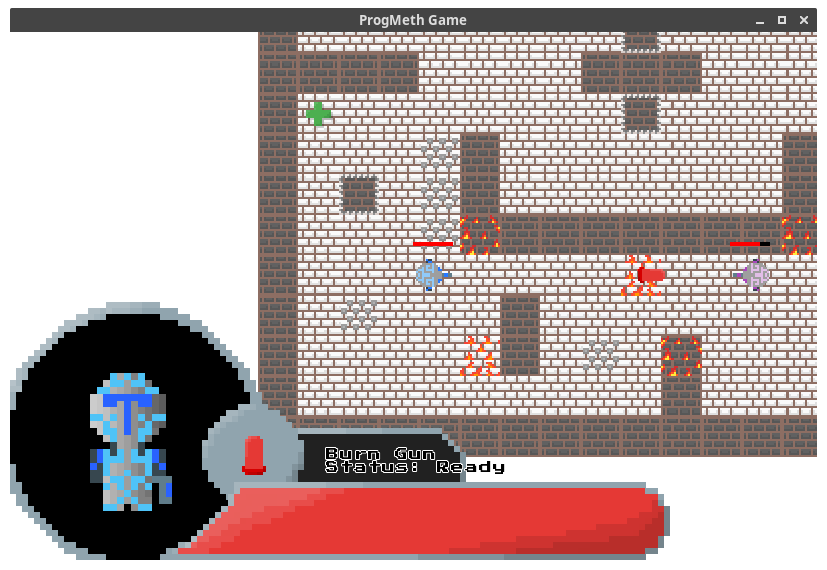
\includegraphics[width=\linewidth]{docasset/shot}
\end{figure}


\textbf{Quick Note:} Jumps to \protect\hyperlink{game-manual}{Game
Manual} now! if you want to play the game.

\textbf{Irritating Crusader} (``The game'') is a two-player, top-down,
shooter game where the player ``disrupt'' the opponent by shooting the
``effect bullets'', eventually causing the other player to ``confuse''
and get killed by the ``traps''.

This report describe the game's gameplay for the players (``Game
Manual'') and also the game's technical overview for developers
(``Technical Description'').

\hypertarget{game-manual}{%
\section{Game Manual}\label{game-manual}}

\hypertarget{introduction}{%
\subsection{Introduction}\label{introduction}}

\textbf{Irritating Crusader} is a simple game where there's only one
goal, To kill \emph{all} other player.

The best way to get introduced to this game is to actually start playing
it. Invite your friend (or find one) and follows \textbf{Quick Start}
guide.

If you played it and somehow got confused, We also provides
documentations on bullets, control, etc. below.

\hypertarget{quick-start}{%
\subsection{Quick Start}\label{quick-start}}

\hypertarget{setting-up}{%
\paragraph{Setting up}\label{setting-up}}

\begin{figure}
	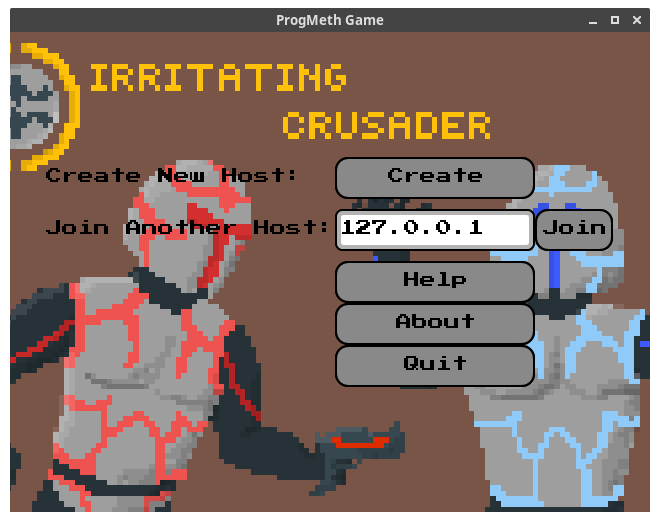
\includegraphics[width=\linewidth]{docasset/welcome}
\end{figure}

\begin{enumerate}
\def\labelenumi{\arabic{enumi}.}
\tightlist
\item
  Grab \texttt{IrritatingCrusader.jar}.
\item
  Install JRE 11 from
  \href{https://www.oracle.com/java/technologies/javase/jdk11-archive-downloads.html}{here}
\item
  If your friends aren't connected to the same local network, Install
  \href{https://www.vpn.net/}{Logmein Hamachi} and follows their guide
  on how to setup a local network.
\end{enumerate}

\hypertarget{playing-the-game}{%
\paragraph{Playing the game}\label{playing-the-game}}

\begin{enumerate}
\def\labelenumi{\arabic{enumi}.}
\tightlist
\item
  Launch \texttt{IrritatingCrusader.jar}.
\end{enumerate}

Have one player be the host and

\begin{enumerate}
\def\labelenumi{\arabic{enumi}.}
\tightlist
\item
  Click \textbf{Create}
\item
  Announce his/her IP to every other players.
\end{enumerate}

Have other players who are not the host do

\begin{enumerate}
\def\labelenumi{\arabic{enumi}.}
\tightlist
\item
  Enter the host's IP and press \textbf{Join}
\end{enumerate}

Once everyone joined the game.\\
Press \texttt{W}, \texttt{A}, \texttt{S}, \texttt{D}, \texttt{Space},
\texttt{E} and see what it do.

\hypertarget{controlling-the-player}{%
\subsection{Controlling the player}\label{controlling-the-player}}

This game is entirely controlled by the keyboard.

\begin{longtable}[]{@{}ll@{}}
\toprule
Keys & Function\tabularnewline
\midrule
\endhead
W & Walk north\tabularnewline
A & Walk west\tabularnewline
S & Walk south\tabularnewline
D & Walk east\tabularnewline
Space & Shoot\tabularnewline
E & Change bullet's type\tabularnewline
\bottomrule
\end{longtable}

But don't walk too much though or you would fall into \textbf{traps}!

\textbf{Note:} There's one key we didn't mention. The \texttt{/} key
opens a cheat console. If you somehow opened it, Close it using
\texttt{ESC} key. Don't cheat!.

\hypertarget{traps}{%
\subsection{Traps}\label{traps}}

\begin{itemize}
\item
  \textbf{Burning Floor:} Make player who step on this type of floor get
  \textbf{Burn} status effect.
\item
  \textbf{Burning Block:} Make player who touch this type of floor get
  \textbf{Burn} status effect.
\item
  \textbf{Spike Trap Floor:} It deal little damage to players who step
  on this type of floor.
\item
  \textbf{Spike Trap Block:} It deal little damage to players who touch
  this type of block.
\item
  \textbf{Curing Floor:} It clear player who step on this type of floor
  their status effects.
\end{itemize}

So now you know how to avoid them, But wouldn't it be good if you can
use them! By shooting \textbf{effect bullets} you can cause other player
to fall into a trap!.

\hypertarget{effect-bullets}{%
\subsection{Effect Bullets}\label{effect-bullets}}

\begin{itemize}
\item
  \textbf{Burn Bullet:} It cause a \textbf{Burn} status effect to the
  target player.
\item
  \textbf{Confuse Bullet:} It cause a \textbf{Confuse} status effect to
  the target player.
\item
  \textbf{Slow Bullet:} It cause a \textbf{Slow} status effect to the
  target player.
\item
  \textbf{Stunt Bullet:} It cause a \textbf{Stunt} status effect to the
  target player.
\item
  \textbf{Hook Bullet:} Move target player to user position.
\item
  \textbf{Teleport Bullet:} Swap location of user and target player.
\end{itemize}

\hypertarget{status-effects}{%
\subsection{Status Effects}\label{status-effects}}

\begin{itemize}
\item
  \textbf{Burn:} Gradually deal damage to plaer who affected by this
  status effect.
\item
  \textbf{Confuse:} Make player who affected by this status effect move
  to the opposite direction of their intention.
\item
  \textbf{Slow:} Make player who affected by this status effect move
  slower.
\item
  \textbf{Stunt:} Make player who affected by this status effect unable
  to move.
\end{itemize}

\hypertarget{hud-status}{%
\subsection{HUD status}\label{hud-status}}

\begin{itemize}
\item
  \textbf{HP bar:} Display your health point.
\item
  \textbf{Gun label:} Display the gun that you are holding.
\item
  \textbf{Bullet label:} Display the bullet from your gun.
\item
  \textbf{Character frame:} Display your character model.
\end{itemize}

\hypertarget{technical-description}{%
\section{Technical Description}\label{technical-description}}

\hypertarget{introduction-1}{%
\subsection{Introduction}\label{introduction-1}}

The game's engine is designed to be a general purpose, multiplayer
shooter engine.\\
The game engine is divided into serveral components and implemented
using external libraries whenever possible.

The following section describes its components and its implementation
detail.

\hypertarget{components}{%
\subsection{Components}\label{components}}

The most complex functionality in the game's engine is the multiplayer
client-server functionality. so the source code's structure is built
around it.

The game consist of two major component. The server and the client.

\hypertarget{the-server}{%
\paragraph{The server}\label{the-server}}

package: \texttt{com.progmethgame.server}

The server is a component that processes the player's input and simulate
the game's law including

\begin{itemize}
\tightlist
\item
  Physic law
\item
  Entity interaction rules
\item
  Entity status reporting.
\end{itemize}

The server then send the resulting calculation (graphic, sound) through
the network

\hypertarget{the-network}{%
\paragraph{The network}\label{the-network}}

package: \texttt{com.progmethgame.network}

The networking is a component that tranparently provides the
client-server communication.

It provides

\begin{itemize}
\tightlist
\item
  Transparent networking system
\item
  Interface for event source and sink.
\item
  Data serialization
\end{itemize}

The networking component then transfer server's data to the client

\hypertarget{the-client}{%
\paragraph{The client}\label{the-client}}

package: \texttt{com.progmethgame.client}

The client is a component that

\begin{itemize}
\tightlist
\item
  Render graphic.
\item
  Play the sound and music
\item
  Send user's keyboard input.
\end{itemize}

The server and the client are both initialized by the launcher

\hypertarget{the-launcher}{%
\paragraph{The launcher}\label{the-launcher}}

package: \texttt{com.progmethgame.launcher}

The launcher is a component that provides GUI for creation and disposal
of the client and the server.

\hypertarget{implementation}{%
\subsection{Implementation}\label{implementation}}

The game engine is implemented using various library.

\hypertarget{graphic-sound-and-controller}{%
\subsubsection{Graphic, Sound and
Controller}\label{graphic-sound-and-controller}}

\textbf{LibGDX} provides graphic, sound and controller library. We
choose this over JavaFX because it

\begin{itemize}
\tightlist
\item
  Provides GL acceleration
\item
  Have many useful utils (eg. Vector arithmetic, Asset management, TMX
  Map loading)
\item
  Comes with boiler plate (eg. Game-loop, Screen management)
\end{itemize}

\hypertarget{networking}{%
\subsubsection{Networking}\label{networking}}

\textbf{KryoNet} provides object serialization and networking system.

\hypertarget{api-documentation}{%
\section{API Documentation}\label{api-documentation}}

Every classes are documented using javadoc. please open
\texttt{javadoc/index.html} with your browser or if you prefer PDF files
please see \texttt{refman.pdf}

\hypertarget{copyright-material}{%
\section{Copyright Material}\label{copyright-material}}

\begin{itemize}
\tightlist
\item
  \textbf{LibGDX} is an Apache2-licensed game engine by Bad Logic Games.
\item
  \textbf{KryoNet} is a networking library by Nathan Sweet licensed
  under BSD-3-Clause.
\item
  \textbf{PressStart2P} is a font by CodeMan38 licensed under Open Font
  License.
\item
  \textbf{plain-james} is a scene2d ui skin by Raymond ``Raeleus''
  Buckley licensed under CC BY 4.0
\item
  \textbf{TMX Format} is a tiled map data format by mapeditor.org
  licensed under CC BY-SA 3.0.
\item
  \textbf{8-bit Game Over} sound effect by Euphrosyyn via freesound.org
  CC BY 3.0
\end{itemize}

\end{document}
